\documentclass[11pt]{article}
\usepackage[utf8]{inputenc}
\usepackage[T1]{fontenc}
\usepackage{mathptmx}
\usepackage[margin=1in]{geometry}
\usepackage{graphicx}
\usepackage{booktabs}
\usepackage{array}
\usepackage{longtable}
\usepackage{authblk}
\usepackage[round]{natbib}
\usepackage{xcolor}
\usepackage[colorlinks=true,allcolors=blue]{hyperref}
\usepackage{titlesec}
\usepackage{caption}
\usepackage{float}
\captionsetup{font=small,labelfont=bf}
\titleformat{\section}{\large\bfseries}{\thesection.}{0.5em}{}
\titleformat{\subsection}{\normalsize\bfseries}{\thesubsection.}{0.5em}{}
\setlength{\parskip}{0.4em}
\setlength{\parindent}{0pt}
\renewcommand{\arraystretch}{1.2}

\title{\bfseries A pre-registered field test of Seismic Frequency Resonance (SFRT)
targeting for orogenic gold: dual-impedance re-analysis, georeferenced structural
integration, and drill-test protocol for the Lac Courville Property, Abitibi, Qu\'ebec}

\author[1]{Aimin Xue}
\author[2]{Ruqing Chen}
\affil[1]{Beijing Petrosound Geoservices Corp., Beijing, China. \texttt{aiminx@126.com}}
\affil[2]{Minesound Ltd., Montreal, Canada. \texttt{ruqing@hotmail.com}}
\date{Pre-registration manuscript --- Part I of a two-part test (predictions filed before drilling)}

\begin{document}
\maketitle

\begin{abstract}
\noindent\textbf{Context.} Claims that a geophysical method ``predicts'' mineralization are
usually published \emph{after} drilling, leaving them open to hindsight bias. We remove that
ambiguity by registering, before any drilling, the targets, drill-hole geometry, and explicit
pass/fail criteria for a single Seismic Frequency Resonance (SFRT) profile (Line~1) over the
Lac Courville gold property, eastern Abitibi greenstone belt, Qu\'ebec.
\textbf{Methods.} We re-process co-located P- and S-wave impedance volumes (Zp, Zs) acquired
along Line~1, compile and georeference the documented gold record of Courville Township from
31 historical assessment reports and a 2021 NI~43-101 report, and integrate the two.
\textbf{Results.} The Zp/Zs ratio --- a density-independent fluid/shear discriminant not used
in the original survey --- defines three sub-line targets, the strongest being T1 (DAS
$\approx$11,500--12,000; 250--550~m). Georeferencing the GM-49463 compilation via its lat/long
graticule lets the Manneville Fault be digitized to UTM (strike N61$^\circ$W); it bounds the
gold corridor $\sim$1.2~km south of Line~1, which therefore sits on the favourable
hanging-wall flank where historical mapping places auriferous branch shears. The NW-trending
(N45$^\circ$W) gold-branch projects onto the northeast-central part of Line~1.
\textbf{Test.} Three 600~m diamond-drill holes (azimuth 225$^\circ$; dips $-58^\circ$ to
$-65^\circ$) are designed to intersect T1--T3. We pre-define a structural-hit criterion
(a shear/altered/veined zone within $\pm$50~m of the predicted depth window) and a
mineralization-hit criterion (Au $\ge$0.3~g/t over $\ge$1~m). Independent QP core logging,
ISO-accredited assaying, and RTK collar survey will adjudicate the outcome in Part~II.
\textbf{Significance.} The design provides a falsifiable, externally witnessed test of whether
SFRT adds value for gold targeting, independent of the result.
\end{abstract}

\textbf{Data and code availability:} all data, processing code, figures and this manuscript
are archived at the project repository (GitHub) with a versioned DOI (Zenodo); see
\S\ref{sec:data}. \textbf{Competing interests:} R.~Chen is affiliated with the property holder
(Minesound Ltd.); A.~Xue is affiliated with the SFRT method provider. The pre-registered
protocol and third-party verification (\S\ref{sec:protocol}) are designed to mitigate this.

\section{Introduction}
Geophysical exploration routinely produces ``targets'' that are later drilled, and the
literature is rich in case studies in which a method is reported to have successfully predicted
mineralization. Because such reports are almost always written after the drill results are
known, they cannot exclude post-hoc rationalisation: targets, tolerances, and success criteria
can be adjusted, consciously or not, to match the outcome. The result is a persistent
credibility gap for newer or proprietary methods, for which an independent, pre-committed test
is rarely available.

This paper is the first of a two-part study designed to close that gap for one method ---
Seismic Frequency Resonance (SFRT) --- on one property. Here (Part~I) we fix, in advance of
drilling, (i) the geological and geophysical basis for three targets, (ii) the drill-hole
geometry that will test them, and (iii) explicit, quantitative criteria by which the test will
be judged a success or a failure. Part~II will report the drill results and adjudicate them
against these criteria without modification. By time-stamping the predictions (\S\ref{sec:data})
we make the test falsifiable in the strict sense: a defined class of drilling outcomes would
count against the method.

We deliberately separate two questions that are often conflated. The first is whether SFRT
images \emph{structure} --- the shear zones, alteration, and competency contrasts that localise
orogenic gold. The second is whether a given imaged structure actually \emph{carries gold} at a
particular intersection, which additionally depends on the local fertility of that structure.
SFRT, like all structurally-vectoring geophysics, can in principle succeed at the first while
failing at the second in any single hole. We therefore register the two criteria separately and
assess them separately.

\section{Regional and district geology}
The Lac Courville Property lies in the southeastern Abitibi Subprovince of the Superior Province,
Canadian Shield, within $\sim$20~km of the Val-d'Or mining camp --- one of the most productive
orogenic-gold districts on Earth. The Abitibi greenstone belt formed in the late Archean
($\sim$2.7~Ga), with the principal gold-forming events at $\sim$2.68--2.67~Ga, and its
greenstone-hosted quartz-carbonate vein deposits are the type examples of the orogenic-gold
class \citep{dube2007}.

The property straddles the northern contact of the \emph{Pascalis-Tiblemont batholith}, a large
multiphase, synvolcanic intrusive complex of diorite, granodiorite and tonalite, against
mafic-to-felsic metavolcanic rocks of the Harricana Group \citep{globex_courville,lafleur2026}.
This contact is occupied by the \emph{Manneville Deformation Corridor}, a regional structure
along the northern margin of the batholith that is associated with numerous gold occurrences and
is interpreted as the eastward continuation of the Manneville Fault
\citep{globex_courville,lafleur2026,bischoff1965}. Stratigraphy and the principal structural
grain trend WNW--ESE; the gold-controlling shears dip steeply to the northeast.

District gold mineralization is structurally controlled and intrusion-hosted: free gold in
quartz (\,$\pm$\,calcite\,$\pm$\,tourmaline) veins and veinlets within silicified, pyritized
diorite and granodiorite, with local chalcopyrite \citep{globex_courville,laverdiere2021}. This
style --- and its setting on a second-order corridor splaying from a crustal-scale break --- is
characteristic of the Val-d'Or orogenic-gold environment \citep{dube2007}.

\section{Property geology and exploration history}
Gold has been documented along the Manneville/Pascalis-Tiblemont corridor immediately northwest
of, and along strike toward, the property for over seventy years. The historical record
(31 Qu\'ebec assessment reports, 1947--2021; compiled in the project repository) establishes a
consistent, structurally-controlled gold system. Key documented endowment includes:
the Pershing-Manitou deposit (45,350~t at 7.9~g/t Au) \citep{beauregard1990};
the Courville Gold Project ``Zone~A'' stockwork (1--7~g/t Au; free gold to $\sim$9~g/t; five
zones $>$0.10~oz/t defined by 1980s drilling), centred $\sim$3.5~km west of the property
\citep{patel1988,laverdiere2021}; and the Uniacke/Obradovich drilling, including hole VC-10
(1.1~ft at 0.68~oz/t, $\approx$23.3~g/t Au) \citep{hawley1994}. Historical mapping traces
gold-bearing porphyry dykes and the Manneville Fault southeastward across the southern part of
the property, south of Lac Courville \citep{bischoff1965}.

Critically for the present test, the 2021 NI~43-101 report on the adjacent Courville Gold
Project concludes that the deposit comprises en-\'echelon veins of limited individual extent and
that the project's principal unresolved problem is an \emph{undefined structural framework} ---
specifically, the absence of an identified major controlling fracture --- and recommends a
dedicated structural study \citep{laverdiere2021}. Imaging crustal-scale shear zones and their
dilational intersections is precisely the information that report identifies as missing, and is
the stated purpose of the SFRT survey analysed here.

\section{SFRT method and Line 1 data}
SFRT is a passive-source seismic technique that uses the frequency-resonance (transfer-function)
response of transmitted waves through solid media to recover wave-impedance variation, a
parameter reported to be more sensitive to lithology and structure than seismic velocity
\citep{xue2020sfrt,xue2023patent}. We treat the method's physical basis as a hypothesis under
test rather than as established, consistent with the falsifiable design of this study.

Line~1 yields co-located P- and S-wave impedance volumes (Zp, Zs), each 176 stations
(DAS 10,000--13,500 at 20~m spacing) by 750 depth samples (0--1498~m at 2~m). Because
Zp $=\rho V_p$ and Zs $=\rho V_s$, the ratio Zp/Zs equals $V_p/V_s$ and is independent of
density, making it a lithology/fluid/alteration discriminant. In the Line~1 data Zp/Zs clusters
at 1.40--1.55 (median 1.43), well below physical rock $V_p/V_s$ (1.7--1.9); the impedances are
therefore \emph{relative} (uncalibrated), and all interpretation uses depth-detrended relative
anomalies rather than absolute values. The composite prospectivity combines relatively low Zp
(alteration/fracture/fluid $\rightarrow$ low velocity), relatively high Zp/Zs (fluid-saturated
shear damage), and high lateral gradient (structural contact / dilational site).

\section{Results: sub-line targets}
The four-panel re-analysis (Fig.~\ref{fig:zpzs}) adds two products absent from the original
single-impedance interpretation: a low-Zs (shearing/fracturing) zone at DAS $\approx$11,700--12,000,
and a strong high-Zp/Zs (fluid/alteration) anomaly at DAS $\approx$11,500--12,000, 250--550~m,
seated on the flank of a competent high-Zp body --- a classic competency-contrast dilation site.
Three targets are defined (Table~\ref{tab:targets}), ranked T1~$>$~T2~$>$~T3. A western
near-surface anomaly (DAS 10,000--10,460, 0--170~m) carries a low score and low Zp/Zs and is
interpreted as an overburden/line-edge effect, not a target.

\begin{figure}[H]
\centering
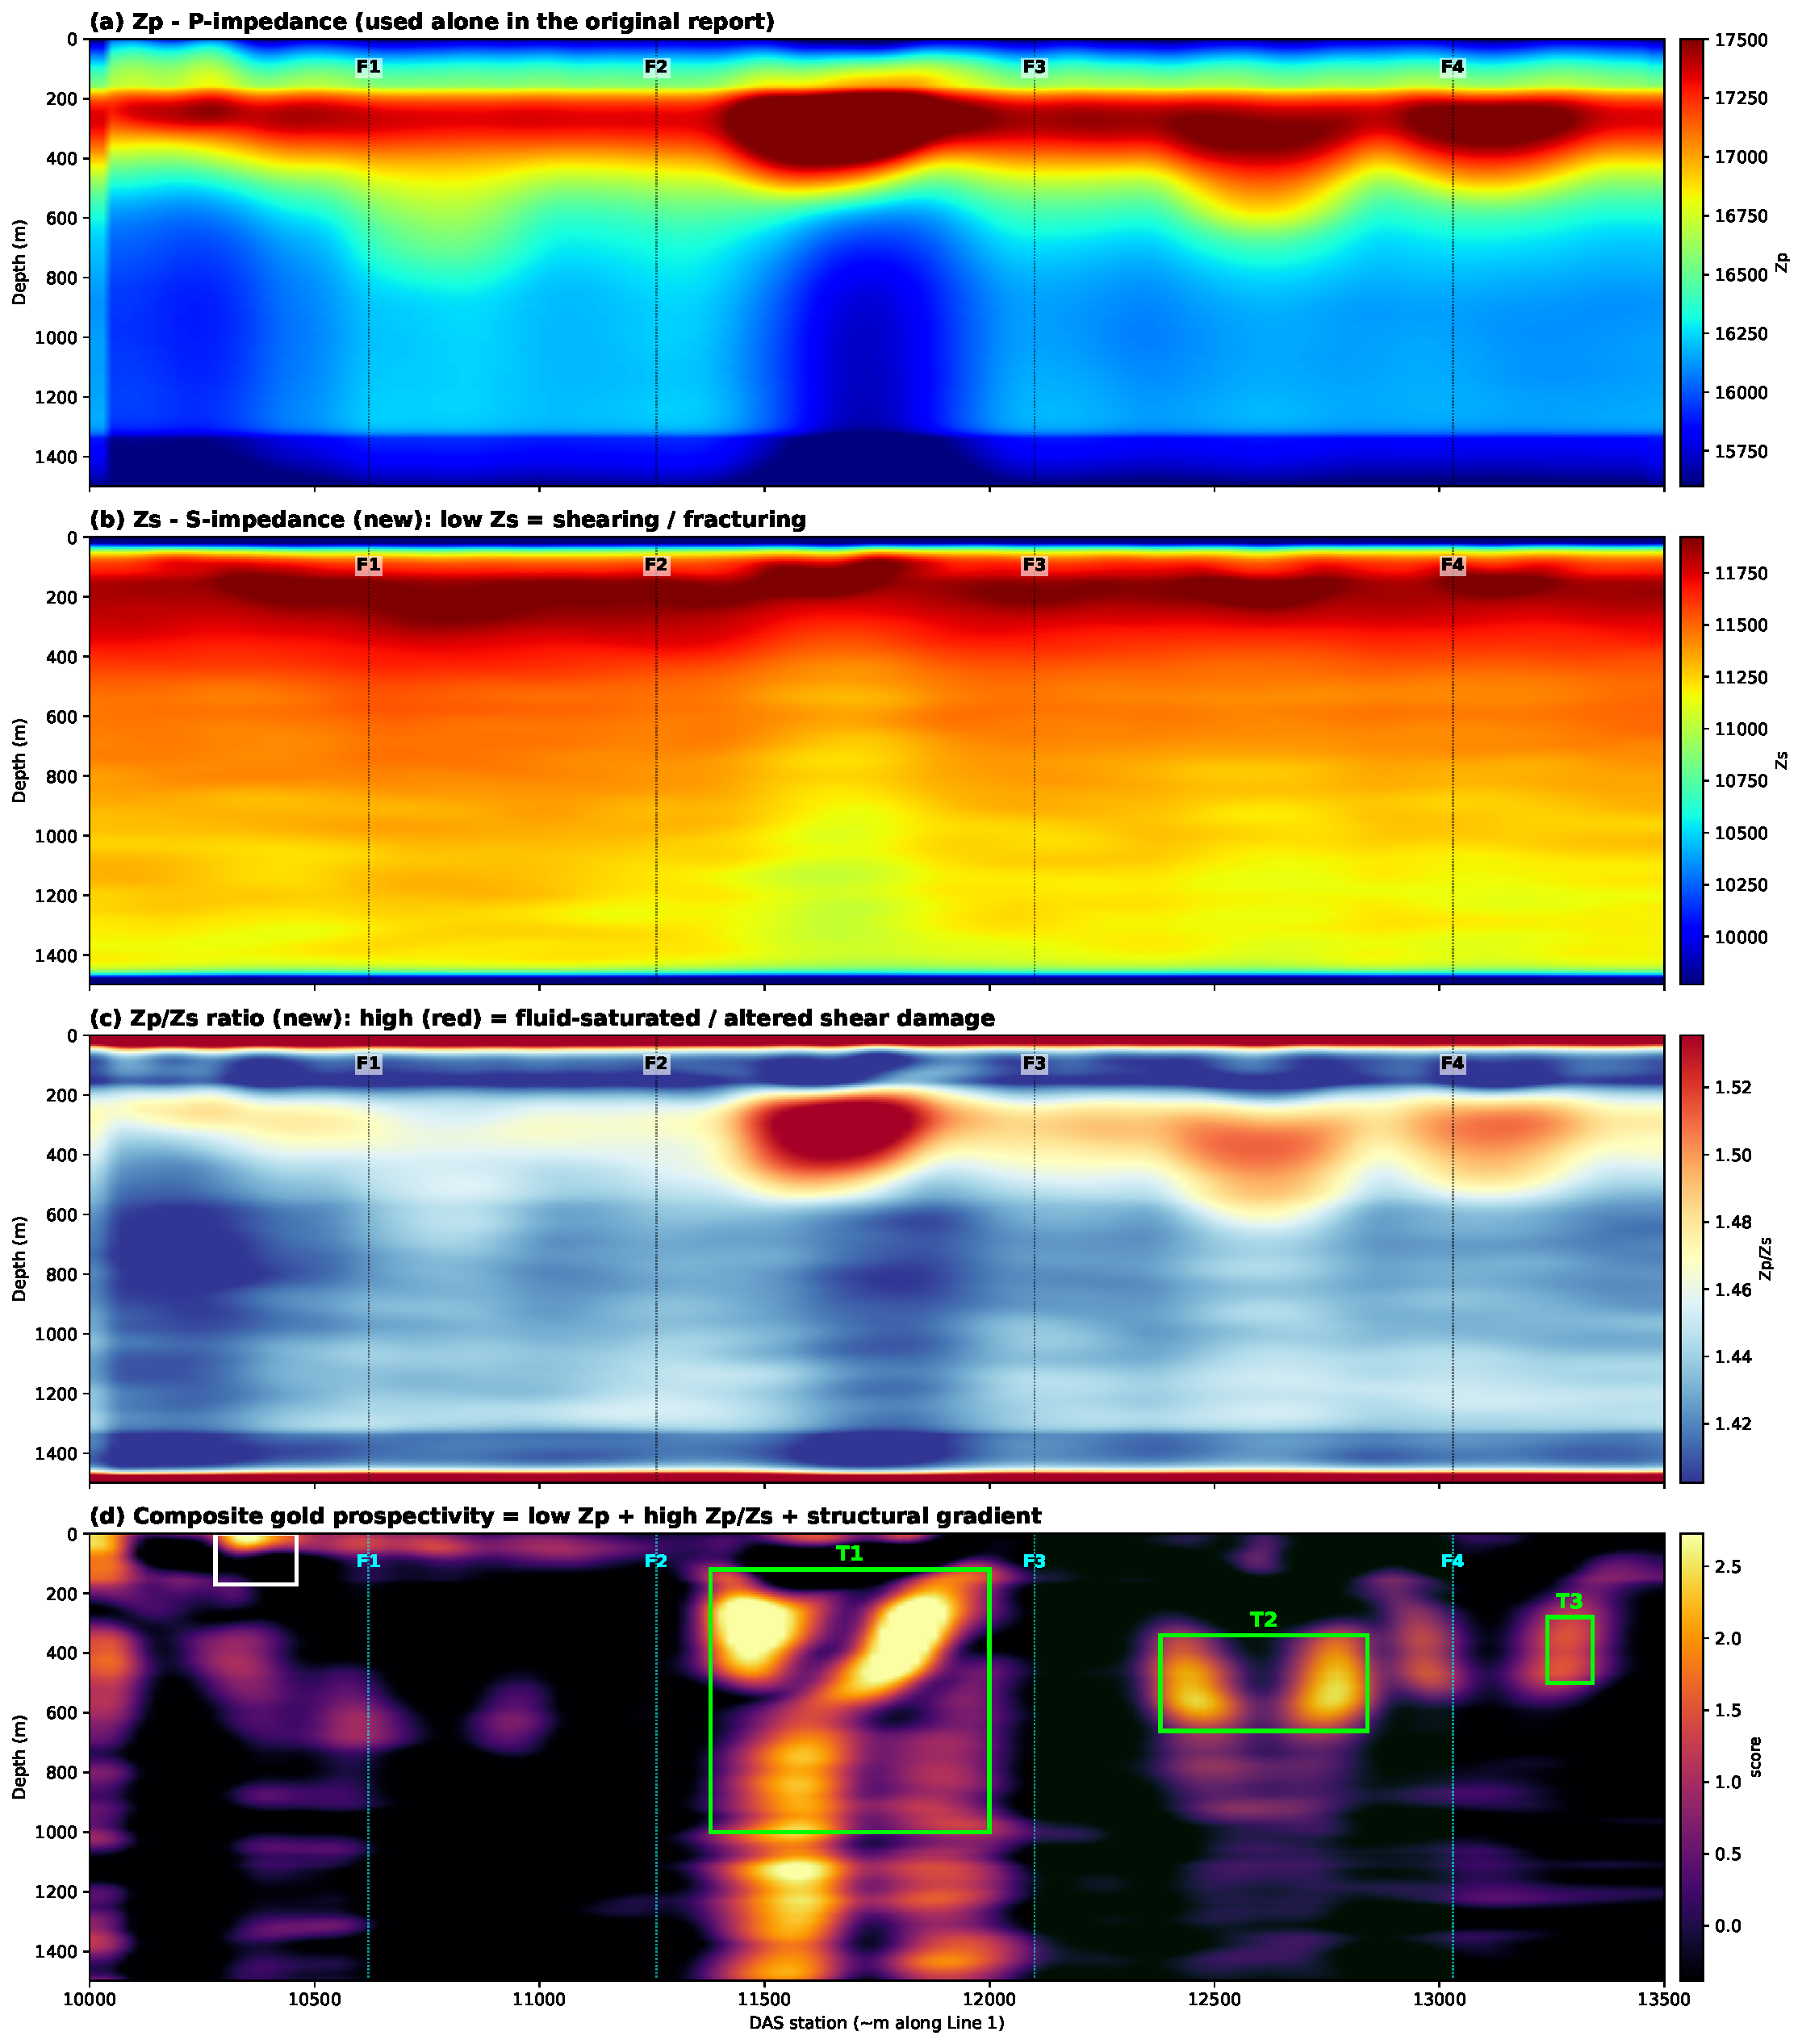
\includegraphics[width=0.60\linewidth]{figures/fig01_zpzs_analysis.pdf}
\caption{Dual-impedance re-analysis of Line~1: (a) Zp; (b) Zs (new); (c) Zp/Zs ratio (new);
(d) composite gold prospectivity with targets T1--T3. Shear zones F1--F4 after the original
report. Impedances are relative (uncalibrated).}
\label{fig:zpzs}
\end{figure}

\begin{table}[t]
\centering\small
\caption{SFRT targets on Line~1 (depth-detrended Zp/Zs anomaly).}
\label{tab:targets}
\begin{tabular}{llllll}
\toprule
Target & DAS & Depth (m) & UTM centre (18N) & $\Delta$(Zp/Zs) & Interpretation \\
\midrule
T1 (primary) & 11,500--12,000 & 250--550 & 326,054 / 5,356,352 & +0.065 & competent-body flank + fluid \\
T2 & 12,380--12,840 & 340--660 & 325,538 / 5,355,632 & +0.045 & F3--F4 corridor \\
T3 & 13,240--13,340 & 280--500 & 325,135 / 5,355,067 & +0.045 & F4 east-flank fault \\
\bottomrule
\end{tabular}
\end{table}

\section{Georeferenced structural integration}
The GM-49463 1:10,000 compilation carries a latitude/longitude graticule (top edge
77$^\circ$30$'$00$''$--77$^\circ$22$'$30$''$ W at 48$^\circ$22$'$30$''$ N). A pixel-to-UTM
transform built from the neat-line corners (reconstructing the NE corner to the metre)
georeferences the map; the principal Manneville lineament, digitized and converted to UTM,
yields a strike of N61$^\circ$W (fit $N=-0.559E+5{,}535{,}051$). The trace runs $\sim$1.2~km
south of Line~1's southwest end (3--4.8~km south of the centre/northeast), so Line~1 lies wholly
on the northern (hanging-wall) flank --- the side on which historical mapping places the
auriferous branch shears \citep{bischoff1965}. The drilled gold centres (Pershing-Manitou,
Zone~A, Uniacke) lie northwest of and along strike toward the property (Fig.~\ref{fig:tie}).
The NW (N45$^\circ$W) gold-branch trend projects onto the northeast-central part of Line~1
(DAS $\approx$10,500--12,000), overlapping the northeast edge of T1. Absolute georeferencing
accuracy is $\sim\pm$100--150~m (NAD27 corner-only graticule, scan distortion, fault curvature).

\begin{figure}[H]
\centering
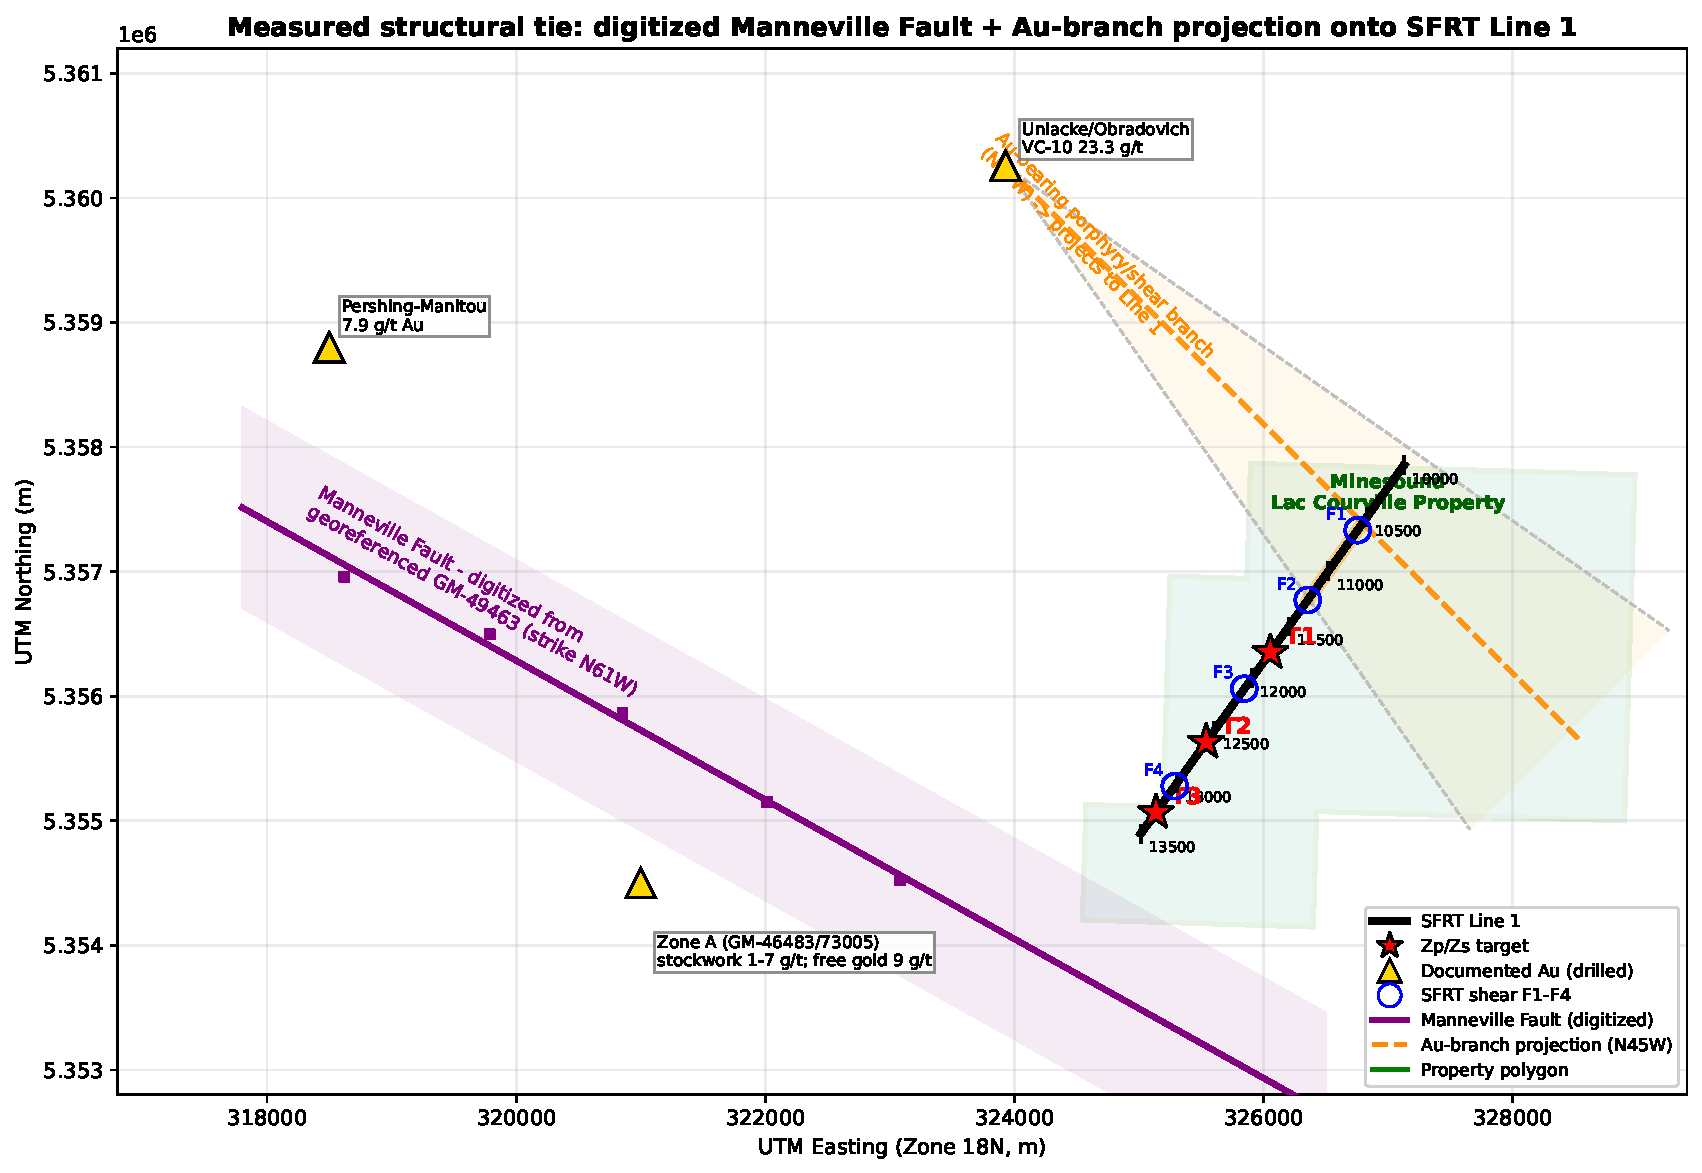
\includegraphics[width=0.96\linewidth]{figures/fig02_structural_tie.pdf}
\caption{Measured structural tie (UTM 18N): digitized Manneville Fault (purple, N61$^\circ$W)
from georeferenced GM-49463; documented gold occurrences; the N45$^\circ$W gold-branch
projection (orange) onto Line~1; property polygon; Line~1 with shear zones F1--F4 and targets
T1--T3.}
\label{fig:tie}
\end{figure}

\section{Pre-drill predictions and falsification criteria}\label{sec:predictions}
We register the following predictions before drilling (Table~\ref{tab:pred}). For each hole the
predicted target is a discrete deformation zone (foliated, quartz-veined) carrying
sericite-carbonate $\pm$ silicification and pyrite $\pm$ chalcopyrite, at the depth window given
by the Zp/Zs target. Two criteria are defined and will be assessed independently:

\textbf{(T1) Structural-hit criterion.} The hole intersects a shear/altered/veined zone within
$\pm$50~m (true vertical) of the predicted depth window.

\textbf{(T2) Mineralization-hit criterion.} Gold $\ge$0.3~g/t over $\ge$1~m occurs within, or
immediately adjacent to ($\le$10~m of), that structural zone.

\textbf{Program-level outcomes (pre-registered).} (a) If $\ge$2 of 3 holes meet the
structural-hit criterion, SFRT is judged effective for \emph{structural} targeting on this line.
(b) If $\ge$1 of 3 holes meets the mineralization-hit criterion, SFRT is judged to show
\emph{direct mineralization vectoring}. (c) If 0 of 3 holes meets the structural-hit criterion,
the test is recorded as a failure of SFRT structural targeting at Lac Courville. A single barren
but structurally-correct intersection does not, by itself, refute the method, because target~T2
addresses structure rather than assured fertility.

\begin{table}[t]
\centering\small
\caption{Pre-registered predictions and pass/fail criteria (filed before drilling).}
\label{tab:pred}
\begin{tabular}{p{2.2cm}p{2.0cm}p{4.6cm}p{4.0cm}}
\toprule
Hole (target) & Predicted depth window & Structural-hit (T1 criterion) & Mineralization-hit (T2 criterion) \\
\midrule
DDH-LC-01 (T1) & 250--550~m & shear/altered/veined zone within $\pm$50~m & Au $\ge$0.3~g/t / $\ge$1~m in or $\le$10~m from the zone \\
DDH-LC-02 (T2) & 340--660~m (tested to 544~m) & shear/altered/veined zone within $\pm$50~m & Au $\ge$0.3~g/t / $\ge$1~m in or $\le$10~m from the zone \\
DDH-LC-03 (T3) & 280--500~m & shear/altered/veined zone within $\pm$50~m & Au $\ge$0.3~g/t / $\ge$1~m in or $\le$10~m from the zone \\
\bottomrule
\end{tabular}
\end{table}

\section{Drilling program and test protocol}\label{sec:protocol}
Three NQ diamond-drill holes of 600~m each are planned (Table~\ref{tab:drill};
Fig.~\ref{fig:section}). All are oriented at azimuth 225$^\circ$ (grid), perpendicular to the
N45$^\circ$W gold-branch strike, with collars northeast of and up-dip from each target so the
hole drills southwest-and-down, cutting the steeply NE-dipping shears at a high angle. Dips
($-58^\circ$ to $-65^\circ$) are chosen so a 600~m hole brackets each target. We note explicitly
that a 600~m hole cannot reach the base of T2 (660~m); DDH-LC-02 therefore tests the
upper-central part of T2 (to $\sim$544~m vertical, which contains the anomaly centroid), and an
extension to $\sim$730~m would be required to test its base. Grid convergence in the area is
$\sim-1.7^\circ$ (true azimuth $\approx$223.3$^\circ$); magnetic declination ($\sim-14^\circ$,
2026) must be applied for compass orientation. Collar elevations will be fixed by RTK survey.

\textbf{Quality assurance and third-party verification.} Core will be logged and signed off by
an independent Qualified Person (Qu\'ebec-registered, NI~43-101 competent). Samples will be
assayed at an ISO/IEC~17025-accredited laboratory (Activation Laboratories, Actlabs) by fire
assay with AA finish (gravimetric finish for high grades), with certified standards, blanks and
duplicates inserted for QA/QC. Collars and hole traces will be surveyed by RTK-GPS. Core will be
photographed and archived. These measures, together with the time-stamped predictions, are
intended to allow external parties to verify the test independently of the authors.

\begin{table}[t]
\centering\small
\caption{Planned drill holes (UTM Zone 18N; azimuth grid; collar elevations to be set by RTK).}
\label{tab:drill}
\begin{tabular}{lllllll}
\toprule
Hole & Target & Collar E & Collar N & Azimuth & Dip & Length \\
\midrule
DDH-LC-01 & T1 & 326,217 & 5,356,515 & 225$^\circ$ & $-60^\circ$ & 600~m \\
DDH-LC-02 & T2 & 325,703 & 5,355,797 & 225$^\circ$ & $-65^\circ$ & 600~m \\
DDH-LC-03 & T3 & 325,307 & 5,355,239 & 225$^\circ$ & $-58^\circ$ & 600~m \\
\bottomrule
\end{tabular}
\end{table}

\begin{figure}[H]
\centering
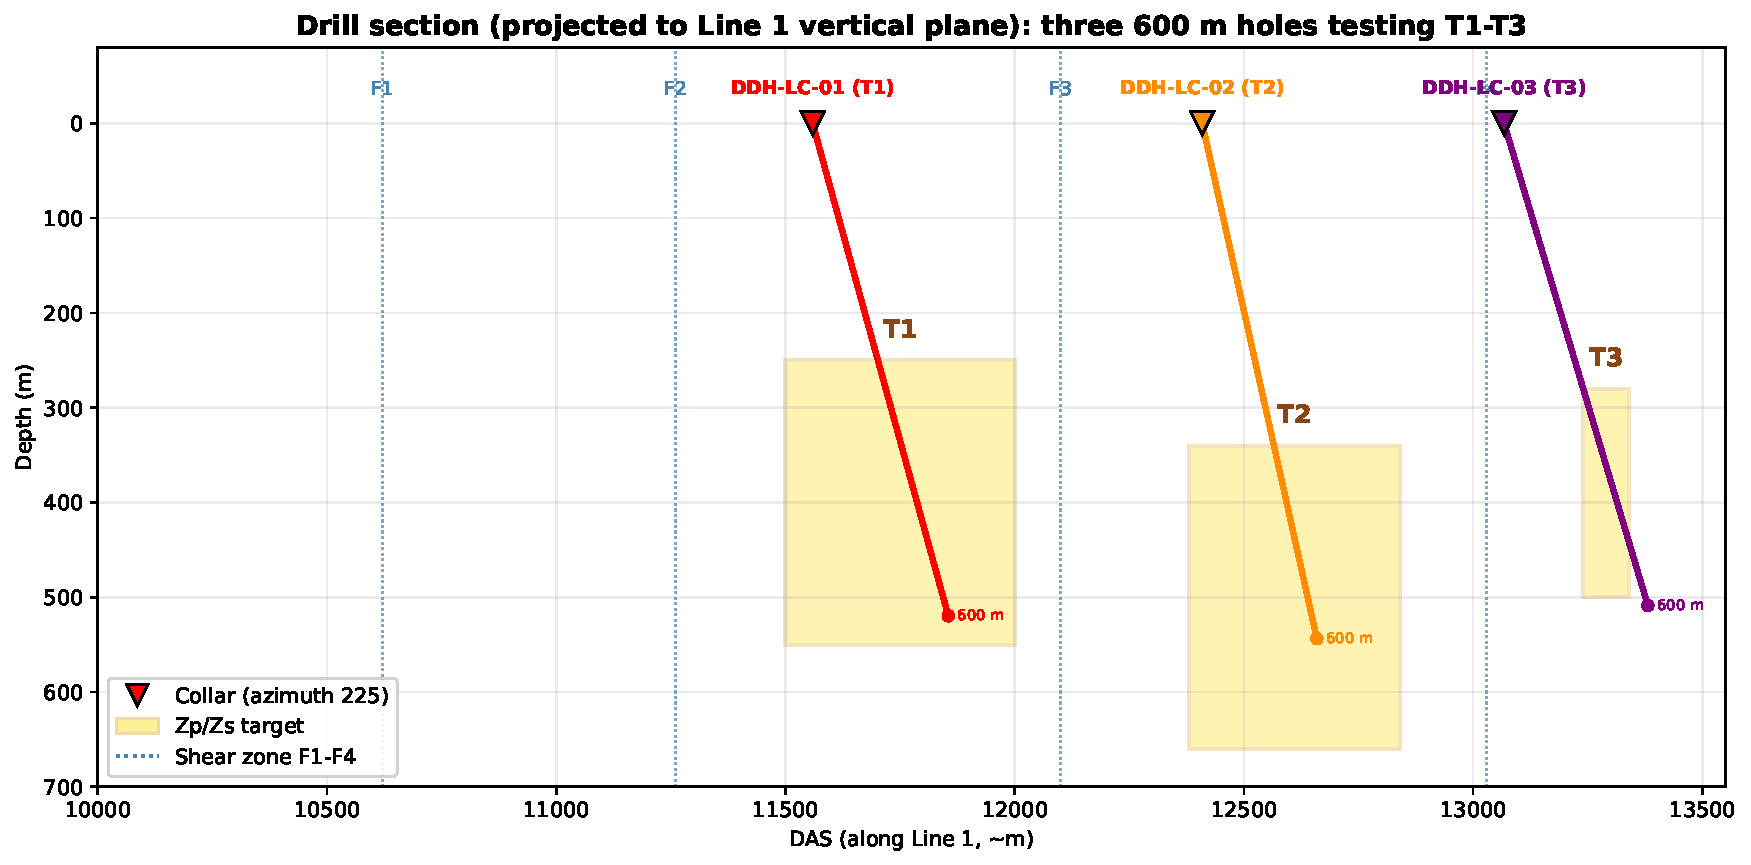
\includegraphics[width=0.96\linewidth]{figures/fig03_drill_section.pdf}
\caption{Drill section projected onto the Line~1 vertical plane: three 600~m holes (collars at
azimuth 225$^\circ$) testing targets T1--T3. Gold boxes are the Zp/Zs targets; dotted lines are
shear zones F1--F4.}
\label{fig:section}
\end{figure}

\section{Discussion}
The test is deliberately conservative in what a positive result can claim. Because Line~1's
impedances are relative, the Zp/Zs anomalies indicate favourable \emph{rock state} (alteration,
fracturing, fluid), not assayed grade; a structural hit is therefore the primary, most defensible
outcome, and mineralization is the more demanding secondary outcome. The single-line geometry
constrains targets in depth and along-line position but not across strike, so a near-miss in the
cross-line direction cannot be excluded for any individual hole; this is one reason the
program-level criteria require a majority of holes rather than relying on one. Absolute
georeferencing of the historical corridor ($\sim\pm$100--150~m) does not affect the on-line
targets, which derive directly from the GPS-located Line~1, but it does limit how precisely the
external gold occurrences can be tied to specific drill intersections.

The principal threat to validity we cannot fully remove is the authors' dual role as property
holder and method provider. We mitigate it structurally: the predictions are time-stamped and
public before drilling; the criteria are quantitative and fixed; and adjudication relies on an
independent QP, an accredited laboratory, and RTK survey rather than on the authors' judgement.
We also commit to reporting Part~II regardless of outcome, including a null result.

\section{Conclusions}
We have re-analysed a single SFRT profile over the Lac Courville Property using the
density-independent Zp/Zs ratio, integrated it with a georeferenced compilation of the district's
documented gold endowment and the digitized Manneville Fault, and used the result to define three
ranked targets and a three-hole, 600~m drill program. Crucially, we register the targets,
drill-hole geometry, and quantitative pass/fail criteria \emph{before} drilling. Part~II will
report the drilling and adjudicate the pre-registered criteria without modification, providing a
falsifiable, externally witnessed assessment of whether SFRT adds value for orogenic-gold
targeting --- an assessment whose credibility does not depend on the outcome.

\section*{Data and code availability}\label{sec:data}
All raw and processed data (impedance volumes, property polygon, targets, drill plan,
predictions, reference ledger), the processing and figure code, the figures, and the
\LaTeX{} source of this manuscript are archived in the project repository
\url{https://github.com/Ruqing1963/lac-courville-sfrt-gold-test} and released with a versioned
DOI on Zenodo at the time of submission, establishing the time-stamp of the pre-registered
predictions.

\section*{Acknowledgments}
We thank the Qu\'ebec Ministère des Ressources naturelles et des For\^ets (SIG\'EOM/EXAMINE) for
open access to the historical assessment-report archive on which the district compilation
depends, and the original authors of those reports, whose work is cited individually in the
repository ledger.

\section*{Author contributions}
A.~Xue developed the SFRT method and acquired/processed the Line~1 data. R.~Chen compiled the
historical record, performed the georeferencing, structural integration and drill design, and
drafted the manuscript. Both authors approved the pre-registered protocol.

\section*{Competing interests}
R.~Chen is affiliated with Minesound Ltd.\ (property holder); A.~Xue is affiliated with the SFRT
method provider. No other competing interests are declared. The pre-registration and
third-party verification described in \S\ref{sec:protocol} are intended to mitigate these
interests.

\bibliographystyle{plainnat}
\bibliography{references}

\end{document}
